\documentclass{article}
\usepackage[T1]{fontenc}
\usepackage{lmodern}
\usepackage{graphicx}
\usepackage{amsmath,amssymb}
\usepackage[a4paper,margin=2cm]{geometry}
\usepackage[absolute,overlay]{textpos}
\setlength{\TPHorizModule}{1mm}
\setlength{\TPVertModule}{1mm}
\usepackage[indonesian]{babel}
\usepackage{hyperref}
\setlength{\emergencystretch}{2em}
% unit: Halaman 65

\begin{document}

% === Halaman 65 (python/native) ===

65

Museum Sandi di Yogyakarta (Sumber: http://museum.lemsaneg.go.id/)

Alamat Jl. Faridan Muridan Noto No. 21, Kota Baru, Yogyakarta. Ini museum san satu-

satunya di Indonesia, bahkan di dunia. Di dalamnya terdapat berbagai koleksi alat sandi 

yang pernah digunakan di Indonesia

% deskripsi: gambar native xref 408
\noindent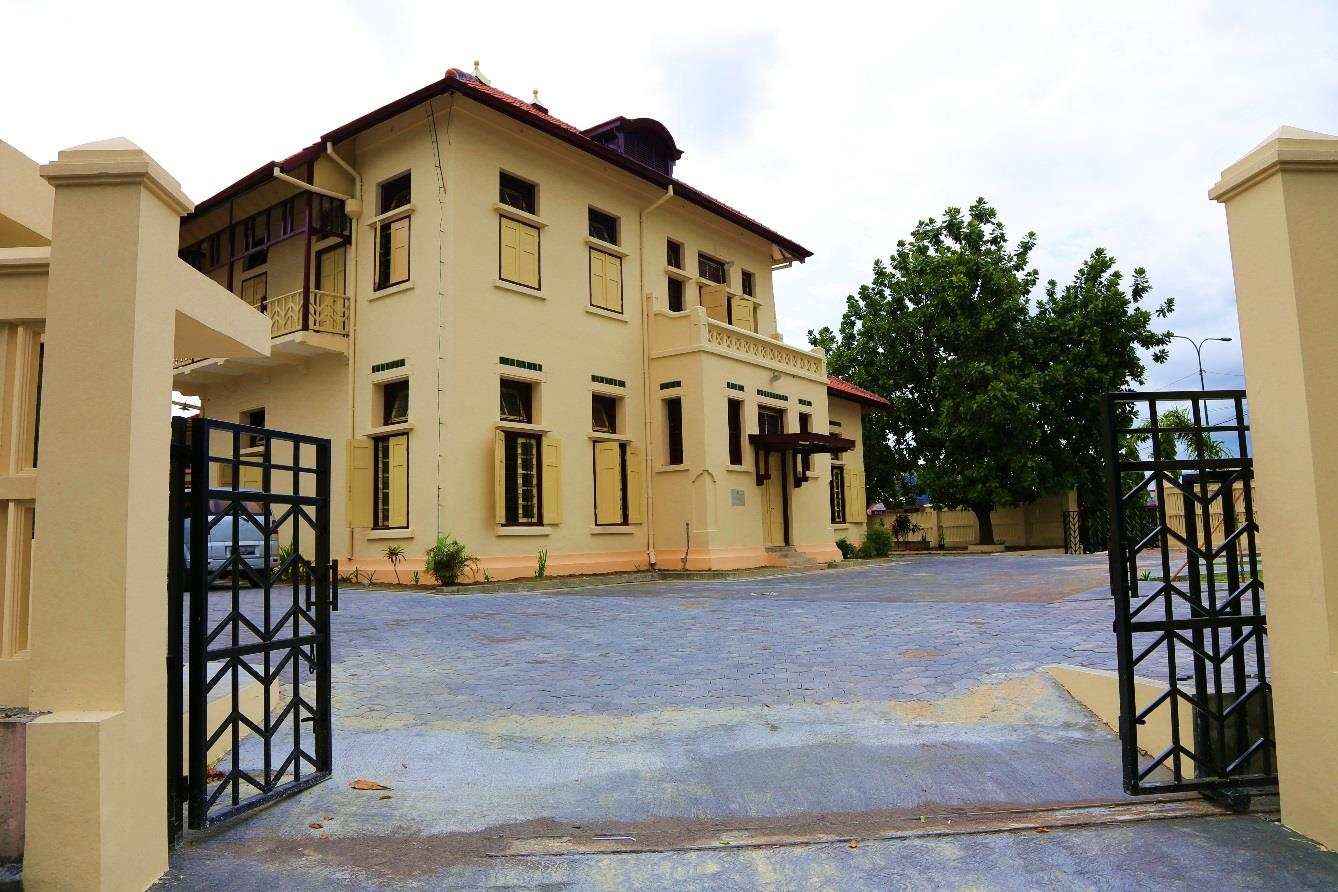
\includegraphics[width=0.85\textwidth]{../../images/python/page_065_img_01.jpeg}

\end{document}
